\section{Split-Plot Designs}

In this section we are going to focus on experimental designs that contain experimental units of different sizes, with different randomizations. These are called \textbf{split-plot designs}.

A split-plot design has a \textbf{whole-plot factor}, treatment scheme was applied to plots, and a \textbf{split-plot factor} where the treatment gets applies to subplots. In the following example the whole-plot factor is \textit{ctrl, new} and the split-plot factor is \textit{A, B, C, D}.

\begin{center}
	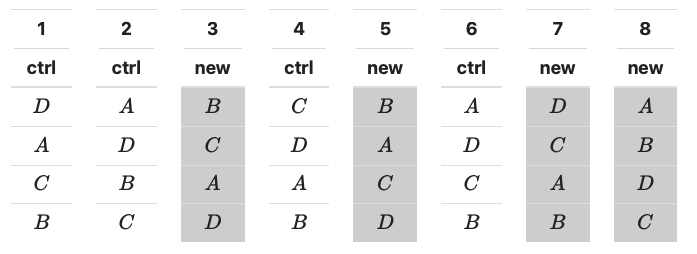
\includegraphics[width=\linewidth]{split-plot.png}
\end{center}

As we now have two different sizes of experimental units, we also need two error terms to model the corresponding experimental errors. One error term acting on the plot level and another one on the subplot level. We end up with the following model:
$$Y_{ijk} = \mu + \alpha_i + \eta_{k(i)} + \beta_j + (\alpha \beta)_{ij} + \epsilon_{ijk}$$

where $\alpha_i$ is the fixed effect of the whole-plot factor and $\beta_{ij}$ is the fixed effect of the split-plot factor. Further $(\alpha \beta)_{ij}$ is the interaction term and $\eta_{k(i)}$, $\epsilon_{ijk}$ are the errors on the plot and subplot level. Note the due to the whole-plot error, observations from the same plot are modelled as correlated data.


\subsection{Properties of Split-Plot Designs}

Typically, split-plot designs are suitable for situations where one of the factors can only be varied on a large scale. For example, fertilizer or irrigation on large plots of land. The price that we pay for this laziness on the whole-plot level is less precision, or less power, for the corresponding main effect because we have much fewer observations on this level. Note that the main effect of the split-plot factor and the interaction between the split-plot and the whole-plot factor are not affected by this loss of efficiency. \medskip

Typical signs for split-plot designs are:
\begin{itemize}
	\item Some treatment factor is constant across multiple time-points, while another changes at each time-point.
	\item Some treatment factor is constant across multiple locations, while another changes at each location.
	\item When planning an experiment: Thoughts like, "It is easier if we do not change these settings too often".
\end{itemize}

If we are not taking into account the special split-plot structure, the results on the whole-plot level will typically be overly optimistic.